\documentclass[12pt]{article}
\usepackage{geometry}
\geometry{a4paper, total={170mm, 250mm}}
\title{\textbf{Homework 3}}
\author{Maedeh Karkhane Yousefi}
\usepackage{float}
\usepackage{graphicx}
\usepackage{subcaption}
\begin{document}
\maketitle
\part*{1.Ballistic Deposition With Relaxation(3.2)}
\paragraph*{}
The goal of this exercise was to make the layer in each time step, as flat as possible.
\paragraph*{}
In order to do so, one way is that the particle check it's two closest neighbors and find the minimum height that it can have after being deposited. So, we actually give the particle a chance to change it's final position for the best. 
\paragraph*{}
I considered a \textit{200$\times$200 Matrix} as the whole system. Each particle have an initial random column and can check it's side columns' heights to decide on it's final to fall into. Afterwards, starting from the bottom, checks each entry for an empty place, respectively. empty and full are differentiated by 0 and other numbers. If the position is empty, the deposition happens and we can move on to the next particle; if not, the particle loops through the array, further. 
\paragraph*{}
I've got 5 functions for the whole operation. The boundary conditions are controlled by returning the first column instead of \textit{column=L+1} and the last column instead of \textit{column=0}, whenever there is a invasion of limits. 
the \textit{height calculator function} loops through rows for the given column, presuming each filled entry as a height increment.
Finally, in the \textit{column choosing function} we have an Ordered Dictionary, which stores these three columns and their heights, respectively, and returns the minimum height. 
\paragraph*{} In order to plot the mean height of a layer in each time step, I introduced a \textit{mean calculator function}, to get the height of each column, in each step, and by using the \textit{mean() function}, return the mean number of each layer. 
\paragraph*{} \textbf{Like what I've written in my previous report}, for this part, we can no longer assume time to be continuous. We shall assume that the time intervals' increment are exponential and therefore, the amount of particles falling between each time interval is increasing exponentially, too. repeating the same procedure, but including this consideration into account, leads us to call the function I've written for calculating the The Standard Deviation at the end of the loop. The \textit{STD function} works like the \textit{mean\underline{\hspace{.08in}} calculater function} except that it returns a list of \textit{std}s.
\paragraph*{} In order to show the the deviation I have set a \textit{run\underline{\hspace{.05in}}num}, by which the code loops through the whole procedure and it creates a list of multiple lists of \textit{std}s. Getting the mean and the std of the same number of elements in every list, we are going to have related std list and mean list to plot the error bar, too. 
\begin{figure}[H]
\centering
	\begin{subfigure}[t]{0.8\textwidth}
		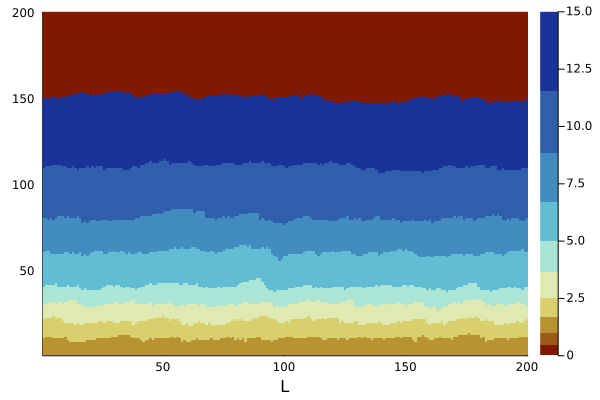
\includegraphics[width=\textwidth]{RandomBallisticDepositionWithRelaxation.png}
		\label{fig:mesh1.1}
		\caption{The dynamics is plotted for n=30000 particles in a \textit{200$\times$200 Matrix}.}
	\end{subfigure}
	\begin{subfigure}[t]{0.45\textwidth}
		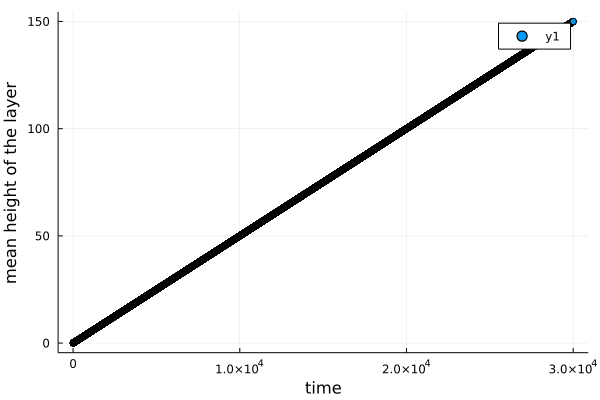
\includegraphics[width=\textwidth]{RandomBallisticDepositionWithRelaxation2.png}
		\label{fig:mesh1.2}
		\caption{The Mean Height of a Layer over Time. Time range is considered to be equal to the whole number of particles(rate=1). n=30000, L=200, slope=0.005. }
	\end{subfigure}\hfill
	\begin{subfigure}[t]{0.45\textwidth}
		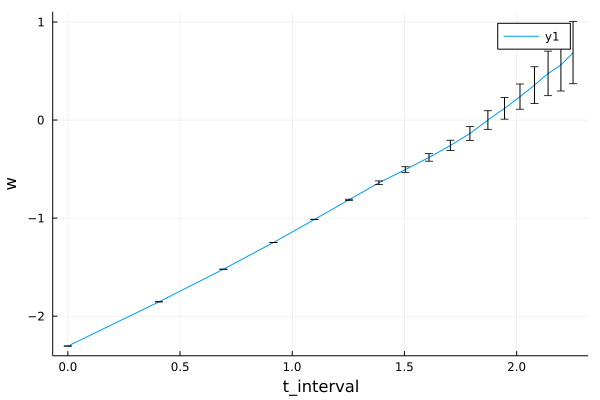
\includegraphics[width=\textwidth]{RandomBallisticDepositionWithRelaxation3.png}
		\label{fig:mesh1.3}
		\caption{w(t) over time. Time intervals are between 1 to 13, increasing by 0.5. The number of falling particles in each time interval are chosen by this time series(n). the code running is repeated for 100 times. $\beta$ equals the slope of the line fit to the plot which is 0.26. Unfortunately the saturation time is not reached in this time range and if I increase the final time, I have runtime problem! So \textit{z} and $\alpha$ are not clear. }
	\end{subfigure}
	\label{fig:mesh1}
	\caption{Plots of Random Ballistic Deposition With Relaxation (exercise3.2)}
\end{figure}
\part*{2. exercise 3.3}
\paragraph*{} Same as the previous exercise we aim to increase the smoothness of the layer in each step. The same boundary conditions is considered in the same structure. After having a particle with a random column, it can choose which height to settle in without changing it's column. So, basically the maximum height is chosen, and if it's the height of neighbors, the particle deposits at the same height, and if it belongs to the same column, particle is falling in, the particle deposits at height plus one. 
\paragraph*{} My \textit{ height calculator function} in this exercise processes quit different, compared with the previous code. Because we have holes in the dynamic, in this code the amount of filled entries no longer represent the height. This is one of the mistakes I made during coding this exercise, assuming everything is the same as the previous one, except for one tiny change. So, in this code I calculated the height by, starting from last row(L) and counting all the empty entries, until reaching the first filled entry. Subtracting the sum of counted empty entries from L, gives the height. 
\begin{figure}[H]
	\centering
	\begin{subfigure}[normal]{0.8\textwidth}
		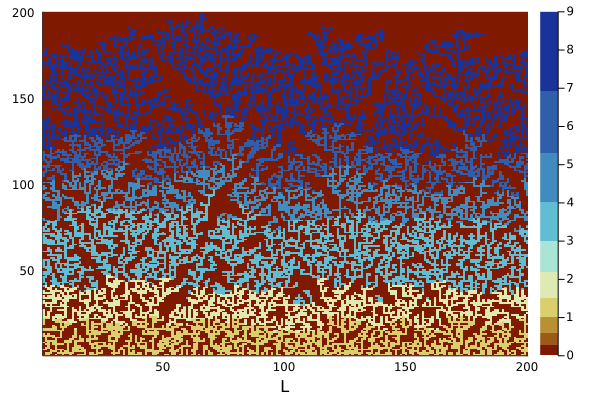
\includegraphics[width=\textwidth]{3.3_1.png}
		\caption{The models dynamic of exercise 3.3. number of particles=30000, L=200, in a \textit{L$\times$L Matrix}.}
		\label{fig:mesh2.1}
	\end{subfigure}
	\begin{subfigure}[t]{0.45\textwidth}
		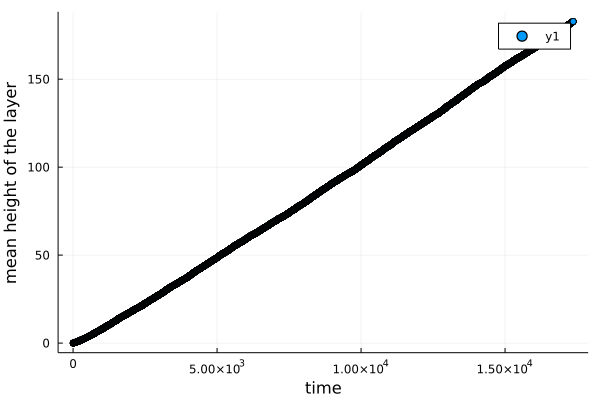
\includegraphics[width=\textwidth]{3.3_2.png}
		\label{fig:mesh2.2}
		\caption{The Mean Height of a Layer over Time. n=30000, L=200, slope=0.01.}
		
	\end{subfigure}\hfill
	\begin{subfigure}[t]{0.45\textwidth}
		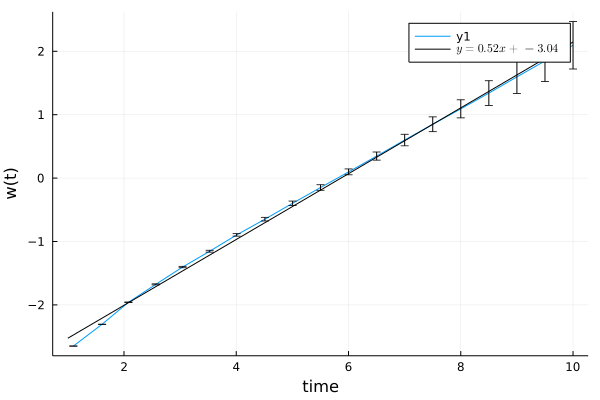
\includegraphics[width=\textwidth]{3.3_3.png}
		\label{fig:mesh2.3}
		\caption{w(t) over time. Time intervals are between 1 to 14, increasing by 0.5. The number of falling particles in each time interval are chosen by this time series(n). the code running is repeated for 100 times. The saturation time is reached after approximately 19 time steps. $t_{s}\sim$ 10.5,$\beta$=0.52, z=0.443797, $\alpha\sim $0.231.}
		\end{subfigure}
	\label{fig:mesh2}
	\caption{plots of exercise 3.3}
\end{figure}
\pagebreak
\part*{3. exercise 3.4}
\paragraph*{} In this exercise I considered the starting point to be at row=1 and column=L/2. Everything in this code is the same as the previous code, except for the fact that no particle with column other than L/2 and height=1 (because in the previous code, it was presumed that if the maximum height doesn't belong to the height of the neighbors, the particle lands on the last particle(which is at the maximum height) can land on the first row.
\begin{figure}[H]
	\centering
	\begin{subfigure}[t]{0.7\textwidth}
		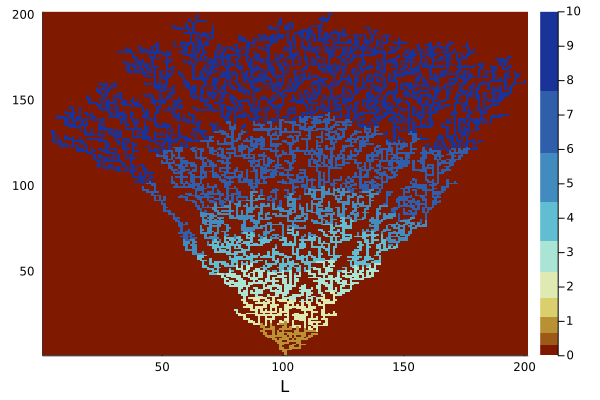
\includegraphics[width=\textwidth]{3.4.png}
		\label{fig:mesh3.1}
		\caption{The models dynamic of exercise 3.4.}
	\end{subfigure}\hfill
	\begin{subfigure}[t]{0.7\textwidth}
		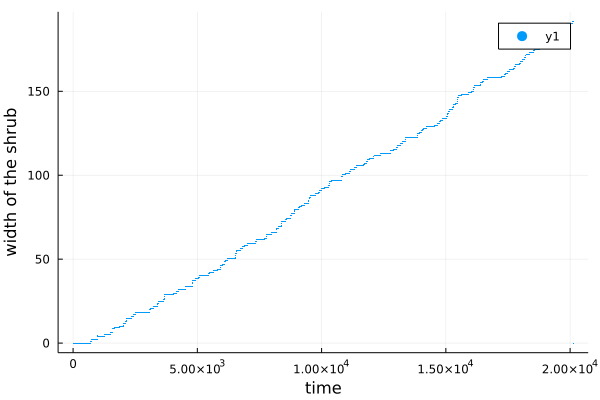
\includegraphics[width=\textwidth]{3.4_width.png}
		\label{fig:mesh3.2}
		\caption{Width of the Shrub over Time. It appears that when time goes on and more particles fall, the width of the tree increases linearly. }
	\end{subfigure}
	\label{fig:mesh3}
	\caption{exercise 3.4. n=30000 particles, L=201, in a \textit{L$\times$L Matrix}}
\end{figure}
\pagebreak
\part*{Percolation }
\part*{4. exercise 4.1}
\paragraph*{} For coding of this exercise I imported \textit{networkx} in \textit{python} to represent percolation in a grid. So instead of what's written in the example, to assume that all the nodes are at first \textit{off} and then each node can become \textit{on} if it's random probability is less than a particular probability, I presumed that all the nodes are initially \textit{on} for simplicity and then some nodes can become \textit{on} with a random probability if the probability is less than a certain \textit{1-P}. 
\begin{figure}[H]
	\centering
	\begin{subfigure}[t]{0.45\textwidth}
		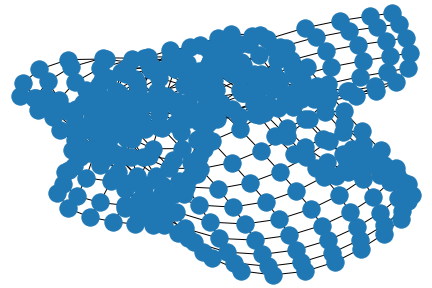
\includegraphics[width=\textwidth]{InitialGraph.png}
		\label{fig:mesh4.1}
		\caption{The Initial Grid with 20 nodes.}
	\end{subfigure}\hfill
	\begin{subfigure}[t]{0.45\textwidth}
		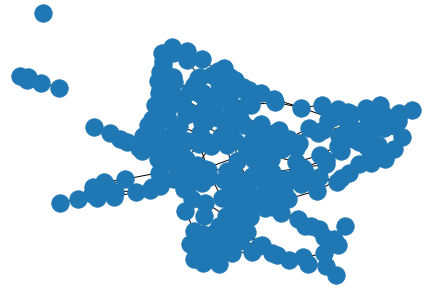
\includegraphics[width=\textwidth]{FinalGraph.png}
		\label{fig:mesh4.2}
		\caption{The Final Grid after some nodes are removed, so that only \textit{on} nodes are left.}
	\end{subfigure}
	\label{fig:mesh4}
	\caption{Figures of the Grid before and after elimination of \textit{off} nodes.The probability that a node can change to \textit{on}  state \textit{(P)}=0.8. For this set of results, there \textit{is} an infinite cluster.}
\end{figure}
\pagebreak
\part*{5. exercise 4.2}
\paragraph*{} The algorithm of this exercise is just like what is written in the book. I considered a \textit{L$\times$L Matrix} with all it's entries set to be initially zero. After setting all the first column's elements to one and the last column's elements to \textit{int\_ max=100000}, the loops go through each elements of the second column to 1-L column, doing everything just as the book has said. \textit{color\_ change\_ list} is the colors of the neighbors or the better to say the attributes of the neighbors that we need to have for the algorithm to work properly. The results are also shown as a gif. Here are some snapshots of them:
\begin{figure}[H]
	\begin{subfigure}[t]{0.3\textwidth}
		\centering
		\includegraphics[width=\textwidth]{p=0.1,A.png}
		\label{fig:mesh5.1}
		\caption{First snapshot for p=0.1.}
	\end{subfigure}\hfill
	\begin{subfigure}[t]{0.3\textwidth}
		\centering
		\includegraphics[width=\textwidth]{p=0.1,B.png}
		\label{fig:mesh5.2}
		\caption{Second snapshot for p=0.1.}
	\end{subfigure}\hfill
	\begin{subfigure}[t]{0.3\textwidth}
		\centering
		\includegraphics[width=\textwidth]{p=0.1,C.png}
		\label{fig:mesh5.3}
		\caption{Third snapshot for p=0.1}
	\end{subfigure}
	\centering
	\label{fig:mesh5}
	\caption{Percolation using coloring algorithm. \textit{100$\times$100 Matrix},int\_ max=100000, p=0.1.}
\end{figure}
\begin{figure}[H]
	\begin{subfigure}[t]{0.3\textwidth}
		\centering
		\includegraphics[width=\textwidth]{p=0.5,A.png}
		\label{fig:mesh6.1}
		\caption{First snapshot for p=0.5.}
	\end{subfigure}\hfill
	\begin{subfigure}[t]{0.3\textwidth}
		\centering
		\includegraphics[width=\textwidth]{p=0.5,B.png}
		\label{fig:mesh6.2}
		\caption{Second snapshot for p=0.5.}
	\end{subfigure}\hfill
	\begin{subfigure}[t]{0.3\textwidth}
		\centering
		\includegraphics[width=\textwidth]{p=0.5,C.png}
		\label{fig:mesh6.3}
		\caption{Third snapshot for p=0.5}
	\end{subfigure}
	\centering
	\label{fig:mesh6}
	\caption{Percolation using coloring algorithm. \textit{100$\times$100 Matrix},int\_ max=100000, p=0.5.}
\end{figure}
\begin{figure}[H]
	\begin{subfigure}[t]{0.3\textwidth}
		\centering
		\includegraphics[width=\textwidth]{p=0.8,A.png}
		\label{fig:mesh7.1}
		\caption{First snapshot for p=0.8.}
	\end{subfigure}\hfill
	\begin{subfigure}[t]{0.3\textwidth}
		\centering
		\includegraphics[width=\textwidth]{p=0.1,B.png}
		\label{fig:mesh7.2}
		\caption{Second snapshot for p=0.8.}
	\end{subfigure}\hfill
	\begin{subfigure}[t]{0.3\textwidth}
		\centering
		\includegraphics[width=\textwidth]{p=0.8,C.png}
		\label{fig:mesh7.3}
		\caption{Third snapshot for p=0.8}
	\end{subfigure}
	\centering
	\label{fig:mesh7}
	\caption{Percolation using coloring algorithm. \textit{100$\times$100 Matrix},int\_ max=100000, p=0.8.}
\end{figure}

\part*{6. exercise 4.3}
\paragraph*{} I used the Hoshen-Keoplman algorithm to code this exercise, following the steps as written in the book. I wrote 4 functions. one for building the array of neighbors, consisting of two neighbors( the left and the upper neighbor, if they are on ). returning this to the percolation function, everything else goes as is said in the book. I had some difficulty writing the Recursion Function for returning the alternative labels associated with remaining entries in the feature, so at last I used a whole different strategy for this function, looping through the \textit{L} array until the index and the amount of the label are equal to each other. At last, I wrote a function to check whether there is a intersect between the first and the last column or not. if there is, it returns \textit{1} to to the \textit{for loop} that evaluates this process with different values of \textit{P}, and repeating it for each probability several times. Finally, we have all the values of each run as a mean and STD number, pushed into the main list. Giving this mean final mean list to the \textit{scatter()}, we can have the plots with error bars gained by the final STD list. 
\begin{figure}[H]
	\begin{subfigure}[t]{0.45\textwidth}
		\centering
		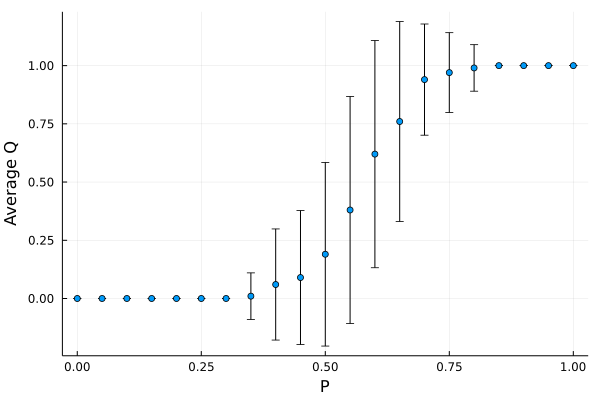
\includegraphics[width=\textwidth]{4.3_L=10.png}
		\label{fig:mesh7.1}
		\caption{L=10, $0 \leq p \leq 1$, $\Delta p=0.05$, number of runs=100.}
	\end{subfigure}\hfill
	\begin{subfigure}[t]{0.45\textwidth}
		\centering
		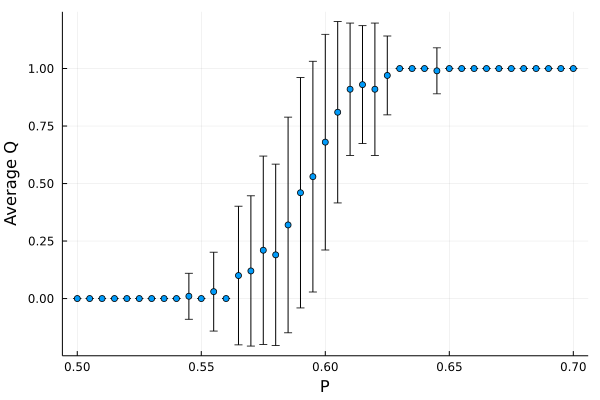
\includegraphics[width=\textwidth]{4.3_L=100.png}
		\label{fig:mesh7.2}
		\caption{L=100, $0.5 \leq p \leq 0.7$, $\Delta p=0.005$, number of runs=100.}
	\end{subfigure}\hfill
	\begin{subfigure}[t]{0.45\textwidth}
		\centering
		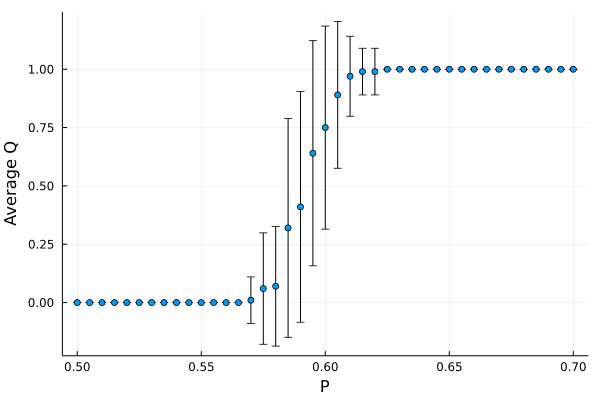
\includegraphics[width=\textwidth]{4.3_L=200.png}
		\label{fig:mesh7.3}
		\caption{L=100, $0.5 \leq p \leq 0.7$, $\Delta p=0.005$, number of runs=100.}
	\end{subfigure}
	\centering
	\label{fig:mesh7}
	\caption{Q per P for different amounts of L. }
\end{figure}

\part*{7. exercise 4.4}
\paragraph*{} To gain these plots, just one tiny change is made in the function that returns the numbers \textit{1} or \textit{0} as an assurance that an intersect exists. We pick a random entry in the matrix and see if it's on and if it's label has a link to the intersect of the first and the last column. if true, then the function returns \textit{1} indicating that the entry is connected to the an infinite cluster. 
\begin{figure}[H]
	\begin{subfigure}[t]{0.45\textwidth}
		\centering
		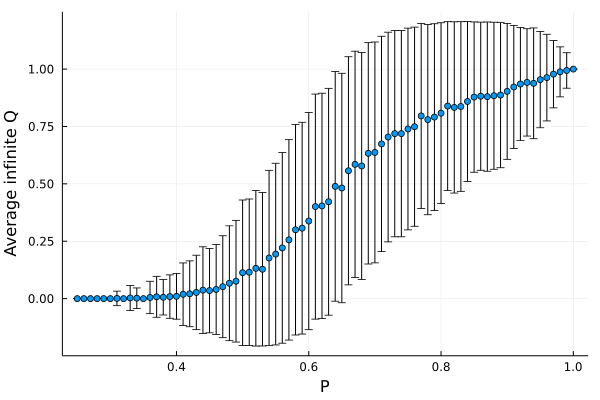
\includegraphics[width=\textwidth]{4.4_L=10.png}
		\label{fig:mesh7.1}
		\caption{L=10, $0.45 \leq p \leq 1$, $\Delta p=0.01$, number of runs=1000.}
	\end{subfigure}\hfill
	\begin{subfigure}[t]{0.45\textwidth}
		\centering
		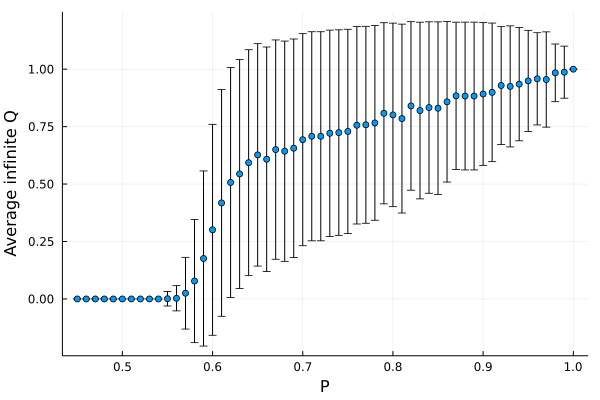
\includegraphics[width=\textwidth]{4.4_L=100.png}
		\label{fig:mesh7.2}
		\caption{L=100, $0.45 \leq p \leq 0.1$, $\Delta p=0.01$, number of runs=1000.}
	\end{subfigure}\hfill
	\begin{subfigure}[t]{0.45\textwidth}
		\centering
		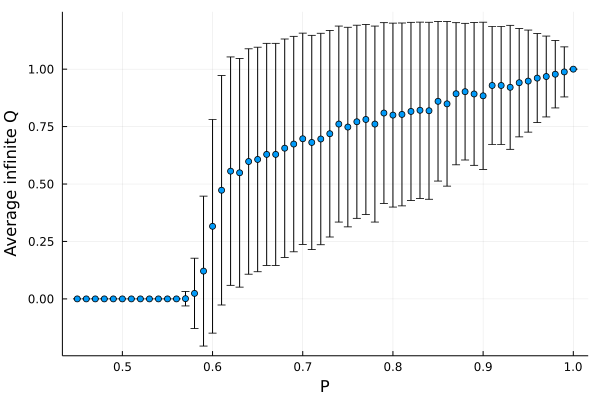
\includegraphics[width=\textwidth]{4.4_L=200.png}
		\label{fig:mesh7.3}
		\caption{L=100, $0.45 \leq p \leq 0.1$, $\Delta p=0.01$, number of runs=1000.}
	\end{subfigure}
	\centering
	\label{fig:mesh7}
	\caption{$Q_{\infty}$ per P for different amounts of L. }
\end{figure}
\end{document}
